%%%%%%%%%%%%%%%%%%%%%%%%%%%%%%%%%%%%%%%%%%%
%%% DOCUMENT PREAMBLE %%%
\documentclass[12pt, a4paper, twoside]{report}
\usepackage[english]{babel}
\usepackage[square,numbers]{natbib}
\usepackage{url}
\usepackage[utf8x]{inputenc}
\usepackage{amsmath}
\usepackage{graphicx}
\usepackage{wrapfig}
\usepackage{parskip}
\usepackage{fancyhdr}
\usepackage{vmargin}
\usepackage[table]{xcolor}
\usepackage{listings}
\usepackage{setspace}
\usepackage{array}
\usepackage{setspace}
\usepackage[colorlinks]{hyperref}
\usepackage{calc}
\usepackage{mwe}
\usepackage{caption}
\usepackage{subcaption}
\usepackage{enumitem}
\usepackage{booktabs}
\usepackage{listings}
\usepackage{wallpaper}
\usepackage{longtable}
\usepackage{float}

\usepackage{caption}
\captionsetup[longtable]{belowskip=-3.3\baselineskip}
\captionsetup[figure]{aboveskip=0.2\baselineskip, belowskip=-1.3\baselineskip}
\captionsetup[wrapfigure]{aboveskip=0.2\baselineskip, belowskip=-1.3\baselineskip}

\bibliographystyle{abbrvnat}

% use it to wrap URI templates 
%\newcommand*{\ptr}[1]{\footnotesize\ttfamily #1}

\newcommand{\cincludegraphics}[2][]{%
	\sbox0{\includegraphics[#1]{#2}}%
	\ht0=\dimexpr\ht0+3pt\relax
	\dp0=3pt
	\splitcell{\box0}%
}
\newcommand{\splitcell}[1]{%
	\begin{tabular}{@{}c@{}}#1\end{tabular}%
}

\let\svparbox\parbox
\renewcommand\parbox[3][c]{\svparbox[#1]{#2}{\strut#3\strut}}

\DeclareTextFontCommand{\ptr}{\footnotesize\ttfamily}
\DeclareTextFontCommand{\texttt}{\footnotesize\ttfamily}

\usepackage[
type={CC},
modifier={by},
version={4.0},
]{doclicense}

\hypersetup{
	colorlinks,
	citecolor=black,
	filecolor=black,
	linkcolor=black,
	urlcolor=black,
	colorlinks=true, %set true if you want colored links
	linktoc=all,     %set to all if you want both sections and subsections linked
%	linkcolor=blue,  %choose some color if you want links to stand out
}
\setmarginsrb{3 cm}{2.5 cm}{3 cm}{2.5 cm}{1 cm}{1.5 cm}{1 cm}{1.5 cm}

\lstset{
	basicstyle=\fontsize{10}{11}\selectfont\ttfamily,
	frame=single,
	breaklines=true,
}

%\graphicspath{{figures/}}

%\title{1}								
%% Title
%\author{Eugeniu Costetchi}						
%% Author
%\date{today's date}
%% Date

%\makeatletter
%\let\thetitle\@title
%\let\theauthor\@author
%\let\thedate\@date
%\makeatother

%\pagestyle{fancy}
%\fancyhf{}
%\lhead{\DelAuthor}
%\rhead{\DelTitle}
%\cfoot{\thepage}

%%%%%%%%%%%%%%%%%%%%%%%%%%%%%%%%%%%%%%%%%%%%
\begin{document}

%%%%%%%%%%%%%%%%%%%%%%%%%%%%%%%%%%%%%%%%%%%%%%%%%%%%%%%%%%%%%%%%%%%%%%%%%%%%%%%%%%%%%%%%%
%Title Page
%%%%%%%%%%%%%%%%%%%%%%%%%%%%%%%%%%%%%%%%%%%%%%%%%%%%%%%%%%%%%%%%%%%%%%%%%%%%%%%%%%%%%%%%%
%!TEX root = deliverable49.tex

%%%%%%%%%%%%%%%%%%%%%%%%%%%%%%%%%%%%%%%%%%%%%%%%%%%%%%%%%%%%%%%%%%%%%%%%%%%%%%%%%%
% First Page
%%%%%%%%%%%%%%%%%%%%%%%%%%%%%%%%%%%%%%%%%%%%%%%%%%%%%%%%%%%%%%%%%%%%%%%%%%%%%%%%%%

% placing a text box at specific position in the page
% usage: \placetextbox{<horizontal pos>}{<vertical pos>}{<stuff>}
% source: https://tex.stackexchange.com/questions/24663/how-to-place-a-floating-text-box-at-a-specified-location-in-page-coordinates
\newcommand{\placetextbox}[3]{% \placetextbox{<horizontal pos>}{<vertical pos>}{<stuff>}
	\setbox0=\hbox{#3}% Put <stuff> in a box
	\AddToShipoutPictureFG*{% Add <stuff> to current page foreground
		\put(\LenToUnit{#1\paperwidth},\LenToUnit{#2\paperheight}){\vtop{{\null}\makebox[0pt][c]{#3}}}%
	}%
}%

% defining the page metadata variables
\newcommand{\DelTitle}{Installation guide for LAM project}
\newcommand{\DelNumber}{WP 1.3.8}
\newcommand{\DelVersion}{1.0}
\newcommand{\DelCorporateAuthor}{???}
\newcommand{\DelAuthor}{Eugeniu Costetchi}
\newcommand{\DelReviewer}{???}
\newcommand{\DelDate}{???}
\newcommand{\DelInitiative}{???}
\newcommand{\DelPreparation}{???}
\newcommand{\DelReaders}{???}
\newcommand{\DelCopyright}{\textsuperscript{\textcopyright} European Union, 2021 }


\pagestyle{empty}


\begin{titlepage}
	\begin{center}

		\begin{center}
			\begin{center}
				\setlength{\tabcolsep}{0pt}
				
\includegraphics[width=0.35\linewidth]{images/logos/EU-OP.png}
			\end{center}

			\ThisLRCornerWallPaper{1}{images/background}

			\vspace{2mm}

		\end{center}
		\vspace{5cm}
		\textbf{{\large \DelInitiative\\}}
		\vspace{2cm}

		\begin{spacing}{2.5}
			\textbf{\Huge \DelTitle}\\ \vspace{2cm}
		\end{spacing}

		\vspace*{\fill}

		\newcolumntype{C}{ >{\arraybackslash} m{3cm} }

	\end{center}
\end{titlepage}

\clearpage


%%%%%%%%%%%%%%%%%%%%%%%%%%%%%%%%%%%%%%%%%%%%%%%%%%%%%%%%%%%%%%%%%%%%%%%%%%%%%%%%%%
% Second Page 
%%%%%%%%%%%%%%%%%%%%%%%%%%%%%%%%%%%%%%%%%%%%%%%%%%%%%%%%%%%%%%%%%%%%%%%%%%%%%%%%%%
\setlength{\headheight}{1cm}
\setlength{\footskip}{18mm}
\addtolength{\textheight}{-\footskip}
\pagestyle{empty}

\clearpage

\vspace*{\fill}

\textbf{\footnotesize \DelPreparation}

\begin{flushleft}
	\begin{table*}[!b]
		\caption*{\large\textbf{Document metadata}}
		\footnotesize
		\begin{tabular}{p{3.6cm}p{\textwidth-5cm}}
			\textbf{Reference}          & \DelNumber: \DelTitle \\
			\textbf{Corporate Author}   & \DelCorporateAuthor   \\
			\textbf{Author}             & \DelAuthor            \\
			\textbf{Reviewers}          & \DelReviewer          \\
			\textbf{Contractor}         & ???        \\
			\textbf{Framework contract} & ???           \\
			\textbf{Work package}       & \DelNumber            \\
			\textbf{Delivery date}      & \DelDate              \\
			\textbf{Suggested readers}  & \DelReaders           \\
		\end{tabular}
	\end{table*}
\end{flushleft}

\placetextbox{0.37}{0.027}{\footnotesize \DelCopyright}

\clearpage
\section*{Abstract}

	Legal Analysis Methodology (LAM) for OP legal data aims to define the semantic aspects of the Publications Office of the European Union (OP) legal data on very specific level. It provides description of the metadata elements meaning, links them to various document types published in Official Journal or on EUR-Lex and describes the rules for attribution of values. It serves as an overarching framework for describing usage of a suite of legal data standards as applied in in their working context. 
	
	LAM plays an important role in the discovery of the EU legal resources (CELLAR, EUR-Lex, OP Portal), which is a central objective for the OP at large. The proper use of LAM leads to a significant decrease in the missing, confusing, incorrect or insufficient data by the stakeholders. In addition, it can increase the data interoperability (by better understanding) and can facilitate automation for legal data at various levels.

    This document provides a working definition of the architectural stance and design decisions that are to be adopted for the LAM data maintenance and dissemination life-cycle and the supporting services. This process is aligned with the semantic asset publication workflow currently employed by the Standardisation Unit (SU) at the Publications Office of the European Union (OP).
\clearpage


%%%%%%%%%%%%%%%%%%%%%%%%%%%%%%%%%%%%%%%%%%%%%%%%%%%%%%%%%%%%%%%%%%%%%%%%%%%%%%%%%%%%%%%%%
\pagestyle{fancy}
\fancyhf{}
\fancyhead[RE]{\slshape\nouppercase{\rightmark}}      % Chapter in the right on even pages
\fancyhead[LO]{\slshape\nouppercase{\leftmark}}     % Section in the left on odd pages
\cfoot{\thepage}

%%%%%%%%%%%%%%%%%%%%%%%%%%%%%%%%%%%%%%%%%%%%%%%%%%%%%%%%%%%%%%%%%%%%%%%%%%%%%%%%%%%%%%%%%


%%%%%%%%%%%%%%%%%%%%%%%%%%%%%%%%%%%%%%%%%%%%%%%%%%%%%%%%%%%%%%%%%%%%%%%%%%%%%%%%%%%%%%%%%

\tableofcontents
\vspace*{\fill}  
\pagebreak

\renewcommand\bibname{References}
\renewcommand{\thesection}{\arabic{section}} % this provides numbering with sections only, without the chapers
%%%%%%%%%%%%%%%%%%%%%%%%%%%%%%%%%%%%%%%%%%%%%%%%%%%%%%%%%%%%%%%%%%%%%%%%%%%%%%%%%%%%%%%%%
% Content sections follow
%%%%%%%%%%%%%%%%%%%%%%%%%%%%%%%%%%%%%%%%%%%%%%%%%%%%%%%%%%%%%%%%%%%%%%%%%%%%%%%%%%%%%%%%% 

\chapter{Introduction}
\label{sec:introduction}
	
	This document provides a working definition of the architectural stance and design decisions that are to be adopted for the asset publication life-cycle process. This process is materialised as the publication workflow and is currently employed by the Standardisation Unit (SU) at the Publications Office of the European Union (PO).
	
	In this document we (a) establish the baseline architecture, supported by  strategic and motivational information; and (b) develop a target architecture guiding the digital transformation processes towards new technologies. This constitutes a natural evolution in response to changing mission needs defined by SU management, and also takes into consideration the strategic directions proposed by the PO, the European Commission (EC) and the European Parliament (EP) as presented below.
	
	\section{Background considerations}
	
	Given the increasing importance of data standards for the EU institutions, a number of initiatives driven by the public sector, industry and academia have been kick-started in recent years. Some have grown organically, while others are the result of standardisation work. Each of these initiatives introduce specific vocabularies, semantics and technologies, resulting in a heterogeneous state of affairs. These differences hamper data interoperability and thus its reuse by the other institutions or by the wider public. This creates the need for a common approach for publishing public reference data and models. Moreover data, which instantiate these public models, available from different sources shall be easily accessed, linked, and consequently reused.
	
	%  involving interinstitutional information exchange schemes, shared models, ontologies and controlled vocabularies
	
	The PSI directive \cite{directive-2019/1024} across the EU calls for open, unobstructed access to public data in order to improve transparency and to boost innovation via the reuse of public data. The reference data maintained and published by the OP has been identified as data with a high-reuse potential \cite{d-high-value-assets}. Therefore, making this data available in machine-readable formats, as well as following the data as a service paradigm, are required in order to maximise its reuse.
	
	In this context, the Publications Office of the European Union maintains and publishes an ever-increasing number of \textit{reference data} which are vital in the context of inter-institutional information exchange. With regards to reference data, the OP provides an ever-increasing number of services to the main institutional stakeholders and with the aim to extend them to a broader public, enabling active or passive participation in the reference data life cycle, standardisation and harmonisation.

	\section{EU trajectory towards public sector linked open data}
	
	European institutions started out to adopt Semantic Web and Linked Data technologies as part of their visions to become data-centred e-government bodies \citep{decission-456/2005/EC,decission-2015/2240}. 
	
	The EU institutions also aim for implementation of a single digital gateway to ``facilitate interactions between citizens and businesses, on the one hand, and competent authorities, on the other hand, by providing access to online solutions, facilitating the day-to-day activities of citizens and businesses and minimising the obstacles encountered in the internal market. The existence of a single digital gateway providing online access to accurate and up-to-date information, to procedures and to assistance and problem-solving services could help raise the users' awareness of the different existing online services and could save them time and expense'' \citep{directive-2018/1724}. This is well in line with earlier established goals for encouraging the open data and the re-use of public sector information \citep{directive-2013/37/EU,directive-2019/1024}.

	Many of the legacy systems used in the EU institutions use XML data format for exchange and document formats governed by the XSD schemes \citep{xsd1.1-spec}. The aim is to evolve technologically so that both existing and new systems are capable to operate with semantic data representations using RDF \citep{rdf11}, OWL \citep{owl2.0,owl2}, SHACL \citep{shacl-spec} and other representations, and serialised at least in RDF/XML \citep{rdf-xml-Beckett:04:RSS,rdf-xml-Schreiber:14:RXS}, Turtle \citep{turtle-Carothers:14:RT} and JSON-LD \citep{spornyjson,sporny2014json} formats.
	
	For this reason, the OP has already been publishing data in RDF format for over a decade using the Cellar repository \citep{cdm-francesconi2015ontology}. Also, the SU, in particular, is committed to publish and disseminate reference data in semantic formats. 
	
	%Next we outline the state of affairs of the SU to describe the context of the current work. 
	
	\section{Target audience}
	\label{sec:audience}
	The target audience for this document comprises the following groups and stakeholders:	
	\begin{itemize}
		\item Management of the SU
		\item Enterprise architects and data governance specialists
		\item Documentalists involved in the reference data life-cycle
		\item Technical staff in charge of operating workflow components
		\item Developers in charge of workflow and component implementation
		\item Third parties using the SU services and data in charge of harmonisation and standardisation of metadata and processes
	\end{itemize}	
	
	\section{Document scope}
	\label{sec:scope}
	
	This document aims to support SU in the transition towards semantic technologies with a particular focus on the architecture of the publication workflow. 
	
	The central use case is to support the asset publication life-cycle detailed in Section \ref{sec:lifecycle-current-stages}. This includes managing the incoming requests, editing the reference assets in VocBench3 system \citep{stellato2017towards,stellatovocbench}, then exporting the RDF data and passing them as input to a set of processes that validate, assess, transform, package and finally publish the assets in Cellar \cite{cdm-francesconi2015ontology}, the semantic repository, which is the main dissemination platform. This use case has been broken down into sub-use cases that are detailed in Section \ref{sec:business-use cases}.
	
	This architecture is also focused on the transition from XML-based asset sources representation to the RDF-based representation along with the resulting implications. This change has a considerable impact on how the asset lifecycle is organised. 
	
	This document will provide a motivational, business and application account of the asset life-cycle workflow. Each of these accounts is limited strictly to the success scenario of the above-mentioned use case and does not include possible extensions and variations.	
	
	There is a series of aspects that were intentionally left out out scope. For example the recommendations related to the data governance both internally within the SU and also externally in relation with partners, stakeholders and clients are not covered. Also, no implementation details are specified for the new components. Little or not account is provided about the data structures and static objects used in the business process or exchanged between the application services. No monitoring or performance measurement systems are foreseen by this architecture, which, in future work shall be considered across across all architectural levels: starting from motivation level key performance indicators (KPI), through business level process monitoring, down to performance measurement of the applications and the infrastructure indicators. 
	
	A high level treatment with only a few details are provided on how the new impact assessment module shall be implemented; how the workflow orchestration engine shall be configured, what process automation service to use, or what technologies could be chosen for that. Such decisions shall be carried out in subsequent steps as additional discussions need to be conducted with the technical team, business team and the sector management. No asset inventory and metadata management system is proposed either, but these needs are only identified as missing and necessary in Section \ref{sec:implementation-application}.
	
	With this scope in mind, we present in the next section what is the general direction that the digital transformation shall take and what is the starting point for it, given the business and technical state of play. 
\section{Requirements}
\label{sec:requirements}

Although Docker can be executed on any platform, for performance and security reasons we recommend using a Linux OS with kernel version 5.4.x or higher. The services have been tested on Ubuntu 20 server.

There is a range of ports that must be available on the host machine as they will be bound to by different docker services. Although the system administrator may choose to change them by changing the values in of specific environment variables. The inventory of pre-configured ports is provided in Table \ref{tab:port-inventory}.

\begin{longtable}[c]{@{}p{3.64cm}p{1.25cm}p{1.25cm}p{1.9cm}p{5cm}@{}}
	\toprule
	Service name  & HTTP port UI & HTTP port API & Mounted volume \\* \midrule
	\endfirsthead
	%
	\multicolumn{5}{c}%
	{{\bfseries Table \thetable\ continued from previous page}}              \\
	\endhead
	%
	\bottomrule
	\endfoot
	%
	\endlastfoot
	%
	LAM validator & 10002       & 10001          &     rdf-validator -shacl-shape          \\* \hline
	LAM Generation Service & 8050         & 4050               &                \\* \hline
	LAM dedicated triple store & 3010                 &          &    lam-fuseki            \\* \hline
	\caption{Port usage inventory}
	\label{tab:port-inventory}                                               \\
\end{longtable}

%	\vfil
The minimal hardware requirements are as follows
\begin{enumerate}
	\item CPU: Dual core 3Ghz
	\item RAM: 8Gb
	\item SDD system: 2Gb
	\item SDD data: 8Gb 
\end{enumerate}

\section{Installation}
\label{sec:installation}

In order to run the services it is necessary to have Docker \citep{docker} service and docker-compose tool installed. To install them follow the instructions provided on the official websites

\begin{enumerate}
	\item Docker - \url{https://docs.docker.com/engine/install}
	\item Docker Compose - \url{https://docs.docker.com/compose/install}
\end{enumerate}

In case you are using Debian-like OS such as Ubuntu, you may simply run the following Bash commands to install and set the appropriate permissions.

\begin{lstlisting}[language=bash,]
sudo apt -y install docker.io docker-compose git make
sudo groupadd docker
sudo usermod -aG docker $USER
newgrp docker
\end{lstlisting}

Please note that the \textit{docker.io} package si installed rather than the \textit{docker-ce} one.

Next, to launch the services, clone the Git repository containing the \textit{docker-compose.yml}, \textit{.env} file and the \textit{Makefile}. 

\begin{lstlisting}[language=bash,]
git clone https://github.com/meaningfy-ws/lam-workflow.git
cd lam-workflow
\end{lstlisting}

You may choose to adjust these files as necessary on your system. Then change directory into the \textit{lam-workflow} folder and Makefile commands to start and stop services will be available. To start services run

\begin{lstlisting}[language=bash,]
make start-services
\end{lstlisting}

To stop the services run 

\begin{lstlisting}[language=bash,]
make stop-services
\end{lstlisting}

Downloading the Docker images will be triggered automatically on first request to start the services.

To start the services using Makefile

\begin{lstlisting}[language=bash,]
make location=</your-custom/shapes/location> validator-set-shacl-shapes
make start-services
\end{lstlisting}

To stop the services using Makefile

\begin{lstlisting}[language=bash,]
make stop-services
\end{lstlisting}

To start services without Makefile first prepare the volume with LinkedPipes ETL configurations file like this

\begin{lstlisting}[language=bash,]
docker rm temp | true
docker volume rm rdf-validator-shacl-shapes | true
docker volume create rdf-validator-shacl-shapes
docker container create --name temp -v rdf-validator-shacl-shapes:/data busybox
docker cp <your-custom/shapes/location>. temp:/data
docker rm temp
\end{lstlisting}

then start the services

\begin{lstlisting}[language=bash,]
docker-compose --file docker/docker-compose.yml --env-file docker/.env up -d
\end{lstlisting}

To stop the services run

\begin{lstlisting}[language=bash,]
docker-compose --file docker/docker-compose.yml --env-file docker/.env down
\end{lstlisting}

The detailed explanation on how to configure them is provided in the Configuration section for each of these services (See Section \ref{sec:rdf-validator-ss}).

\section{Usage}
\label{sec:usage}

After running the following \texttt{make} command:

\begin{lstlisting}[language=bash,]
make start-services
\end{lstlisting}

described in detail in Section \ref{sec:installation}, all services will be available at either \texttt{localhost} or your configured domain name. The specific ports for each service are specified in table \ref{tab:port-inventory}. 

The following explanation of usage for the services assumes that you have access to \texttt{localhost}. 

\subsection{LAM Validator}
\subsubsection{API}
To access the online documentation and testing grounds for the LAM Validator API service visit the following link \url{http://localhost:10001/ui}. You'll be greeted with an interface like in Figure \ref{fig:validator-api-documentation}.

\begin{figure}[H]
  \centering
  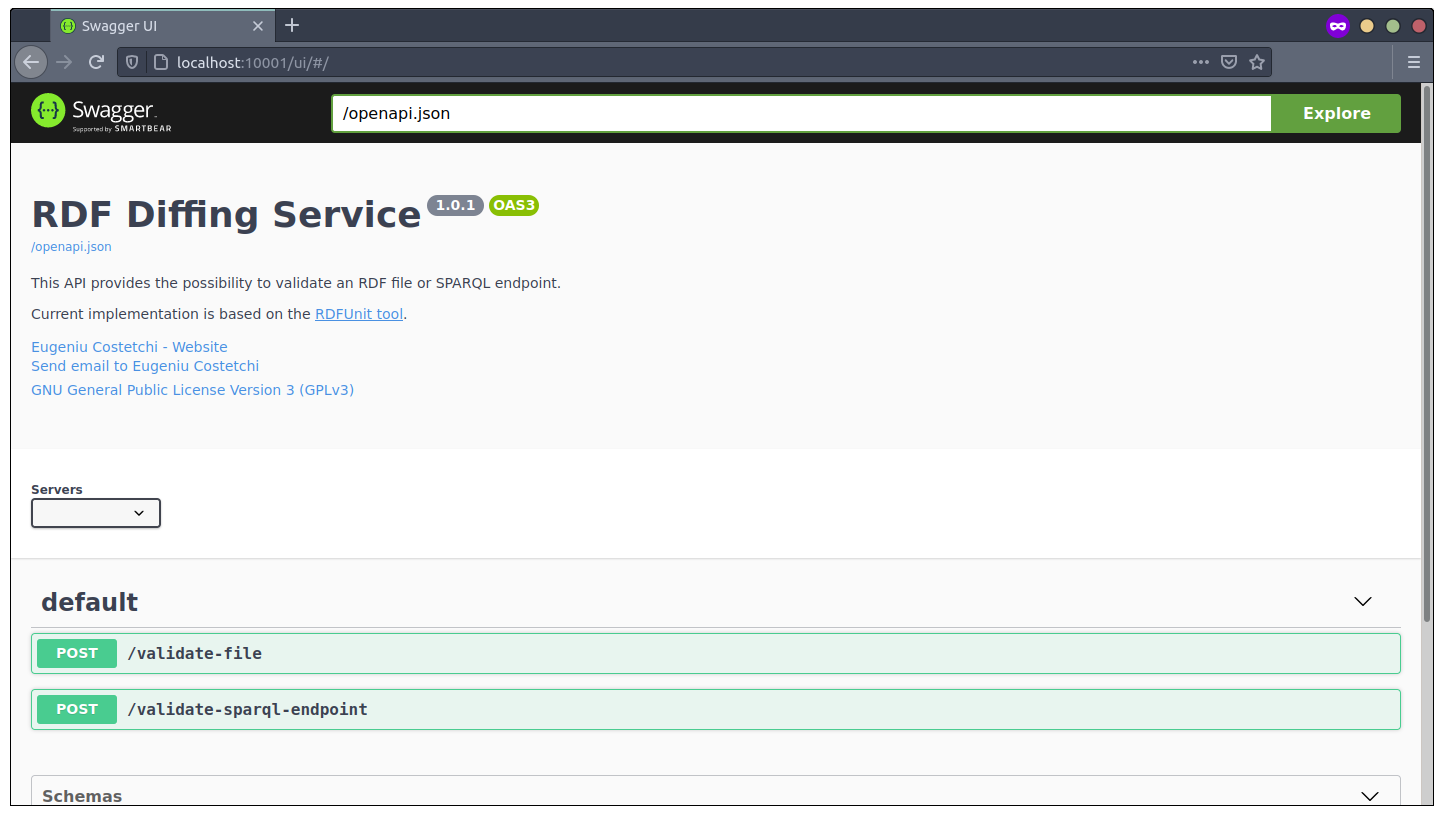
\includegraphics[width=0.9\textwidth]{images/usage/validator-api.png}
  \caption{LAM Validator API documentation}
  \label{fig:validator-api-documentation}
\end{figure} 

Here you can find the defintion for each API endpoint, the HTTP methods, request structure, and the possibility to test the endpoints.

\subsubsection{UI}
To access validation UI visit the following link url{http://localhost:10002}. You'll be greeted with an interface like in Figure \ref{fig:validator-ui-home}.

\begin{figure}[H]
  \centering
  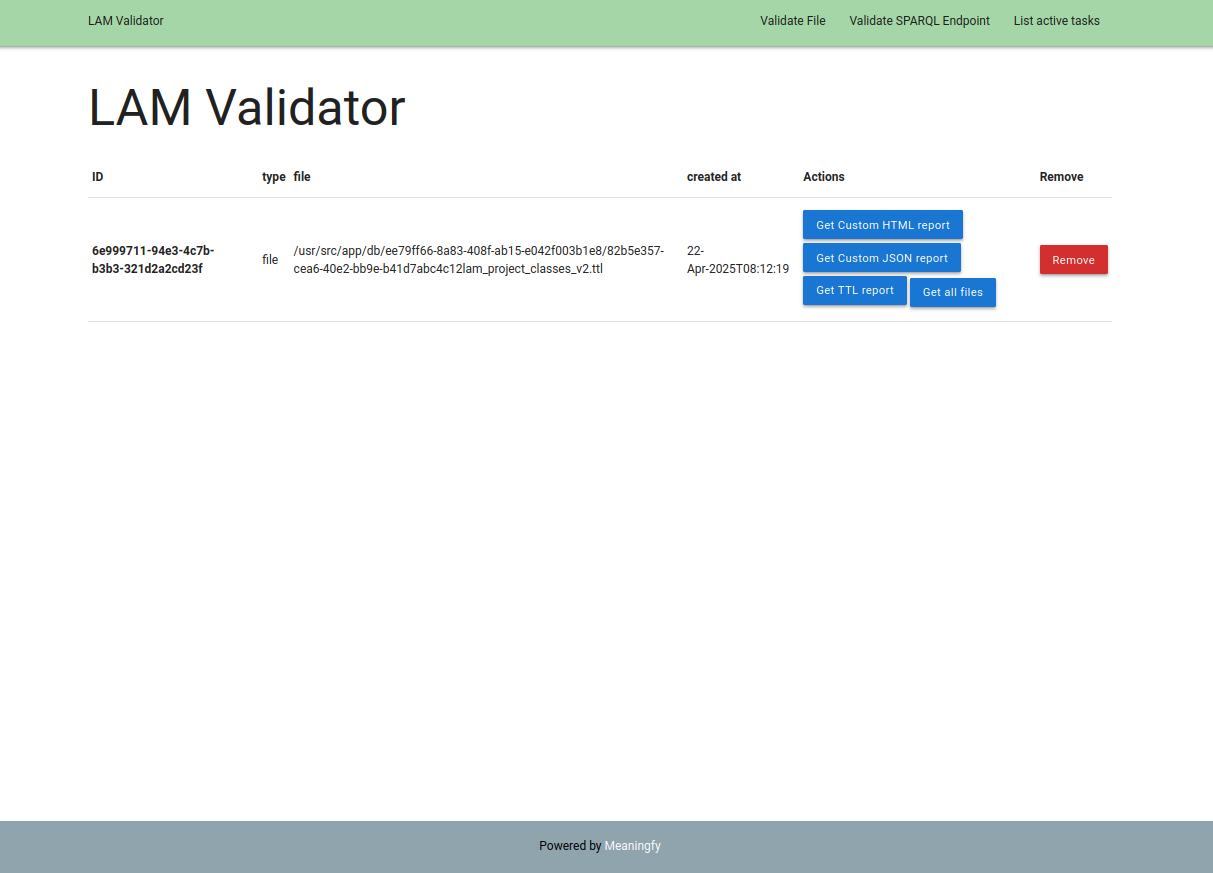
\includegraphics[width=0.9\textwidth]{images/usage/validator-ui-home.png}
  \caption{LAM Validator UI home page}
  \label{fig:validator-ui-home}
\end{figure}

To access the user interface for the LAM Validator service visit the following link \url{http://localhost:10002/validate/shapes/file}. You'll be greeted with an interface like in Figure \ref{fig:validator-ui-file} containing 2 pages.

\begin{figure}[H]
  \centering
  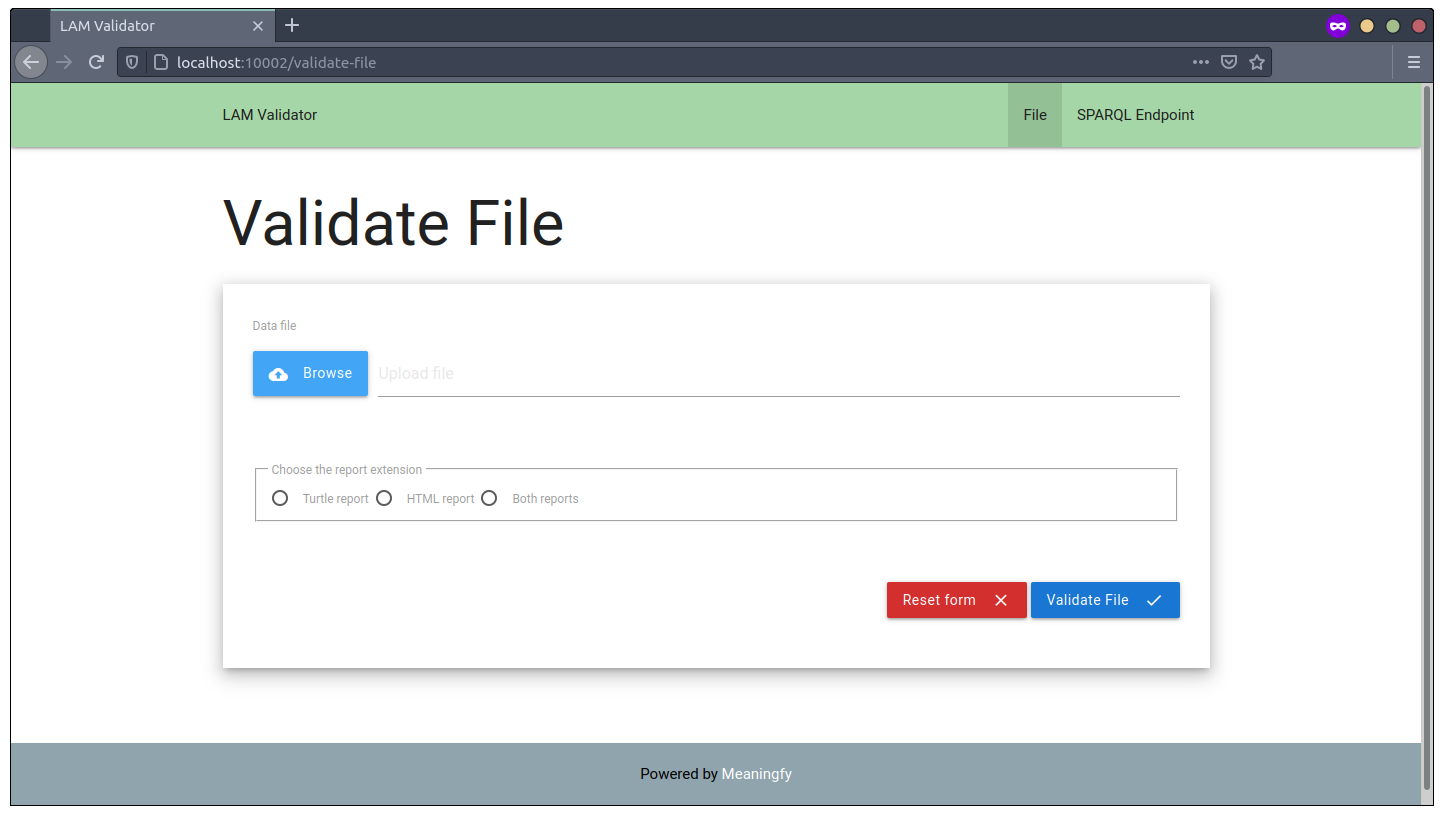
\includegraphics[width=0.9\textwidth]{images/usage/validator-ui-file.png}
  \caption{LAM File Validator UI page}
  \label{fig:validator-ui-file}
\end{figure} 

Here you can access the services for file validation (Figure \ref{fig:validator-ui-file}) and SPARQL endpoint validation (Figure \ref{fig:validator-ui-sparql}).

\begin{figure}[H]
  \centering
  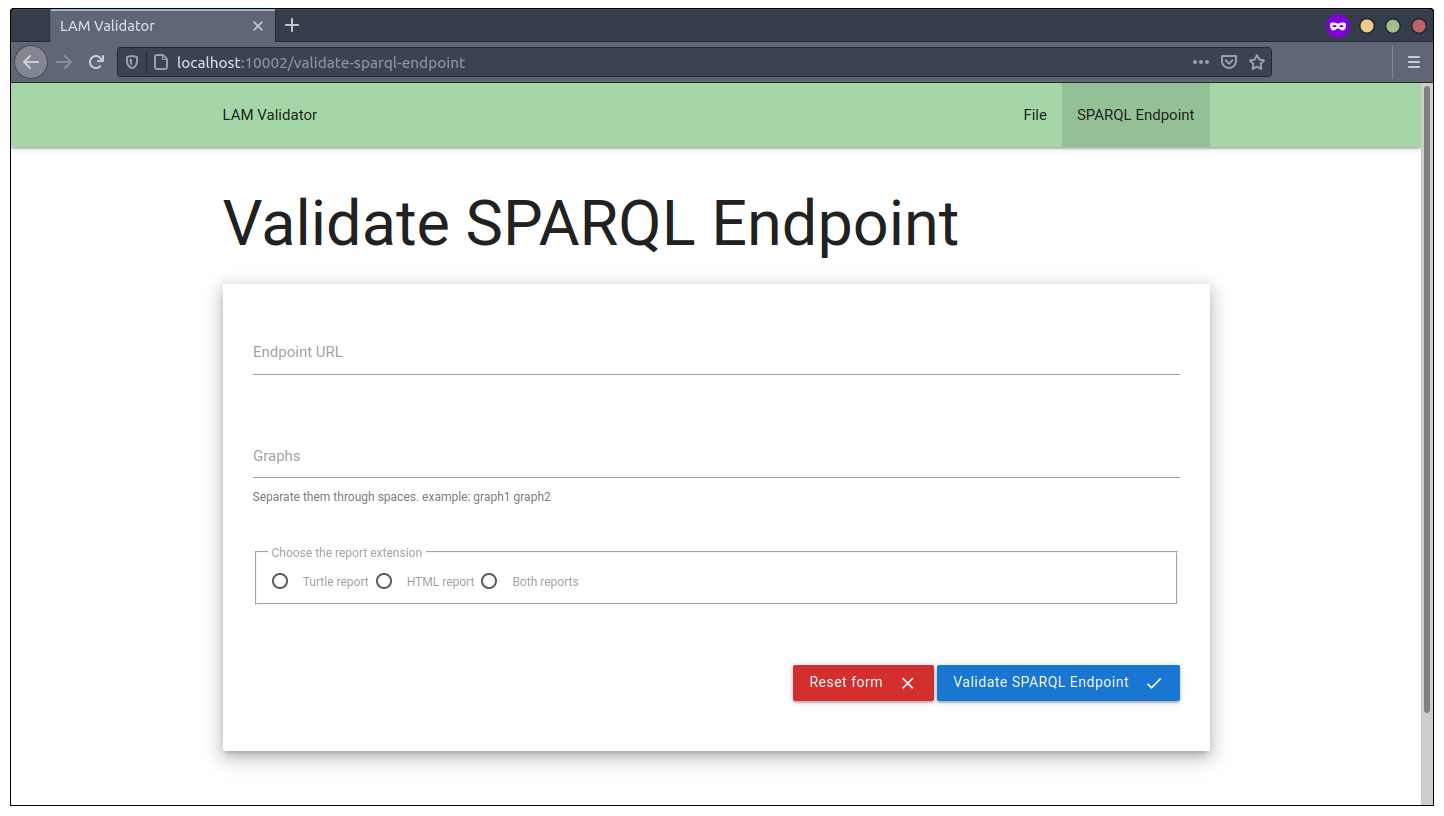
\includegraphics[width=0.9\textwidth]{images/usage/validator-ui-sparql.png}
  \caption{LAM SPARQL Endpoint Validator UI page}
  \label{fig:validator-ui-sparql}
\end{figure} 

\subsection{LAM Generation Services}
\subsubsection{API}
To access the online documentation and testing grounds for the LAM Generation Services API service visit the following link \url{http://localhost:4050/ui}. You'll be greeted with an interface like in Figure \ref{fig:lam-generation-api-documentation}.

\begin{figure}[H]
  \centering
  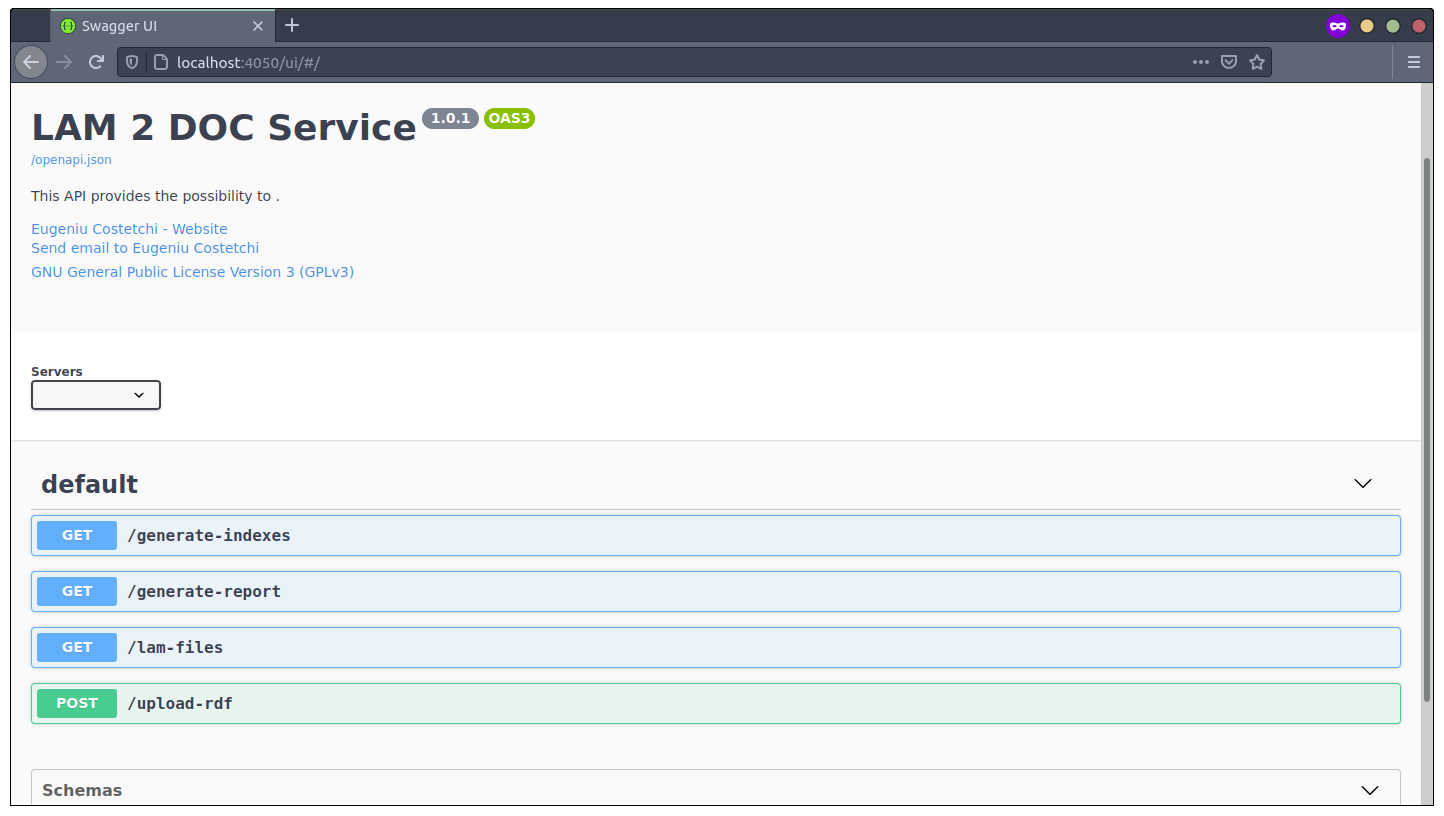
\includegraphics[width=0.9\textwidth]{images/usage/lam-generation-api.png}
  \caption{LAM Generation Services API documentation}
  \label{fig:lam-generation-api-documentation}
\end{figure} 

Here you can find the defintion for each API endpoint, the HTTP methods, request structure, and the possibility to test the endpoints.

\subsubsection{UI}
To access the user interface for the LAM Generation Services visit the following link \url{http://localhost:8050}. You'll be greeted with an interface like in Figure \ref{fig:lam-generation-ui-home} containing 2 pages.

\begin{figure}[H]
  \centering
  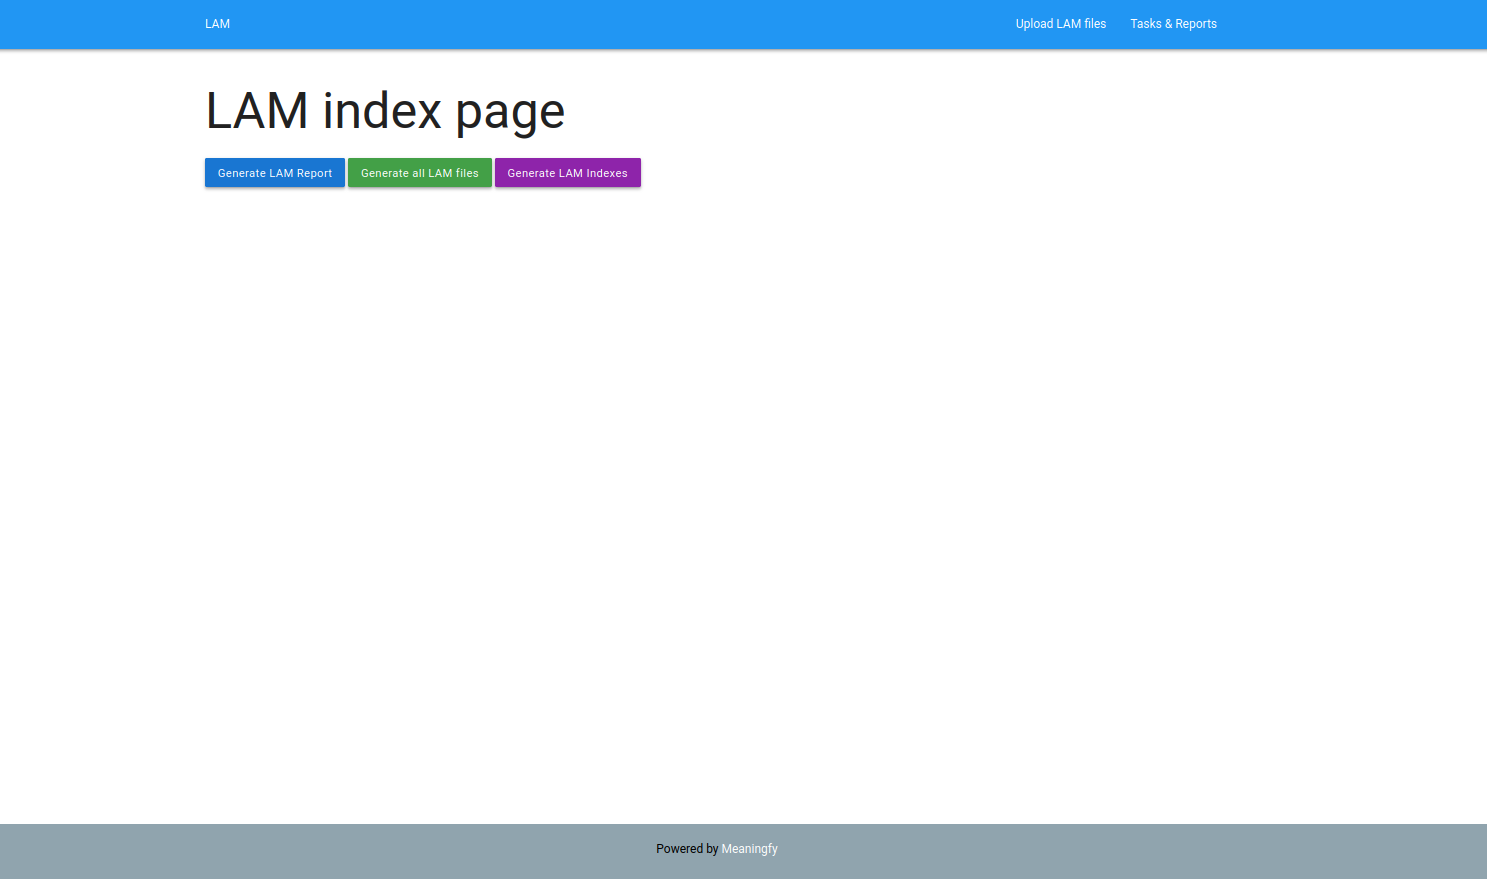
\includegraphics[width=0.9\textwidth]{images/usage/lam-generation-ui-home.png}
  \caption{LAM Generation Services home page}
  \label{fig:lam-generation-ui-home}
\end{figure}

Here you can request the LAM report in 2 formats (Figure \ref{fig:lam-generation-ui-report}), the LAM indexes, or both report formats and indexes in a zipped format.

\begin{figure}[H]
  \centering
  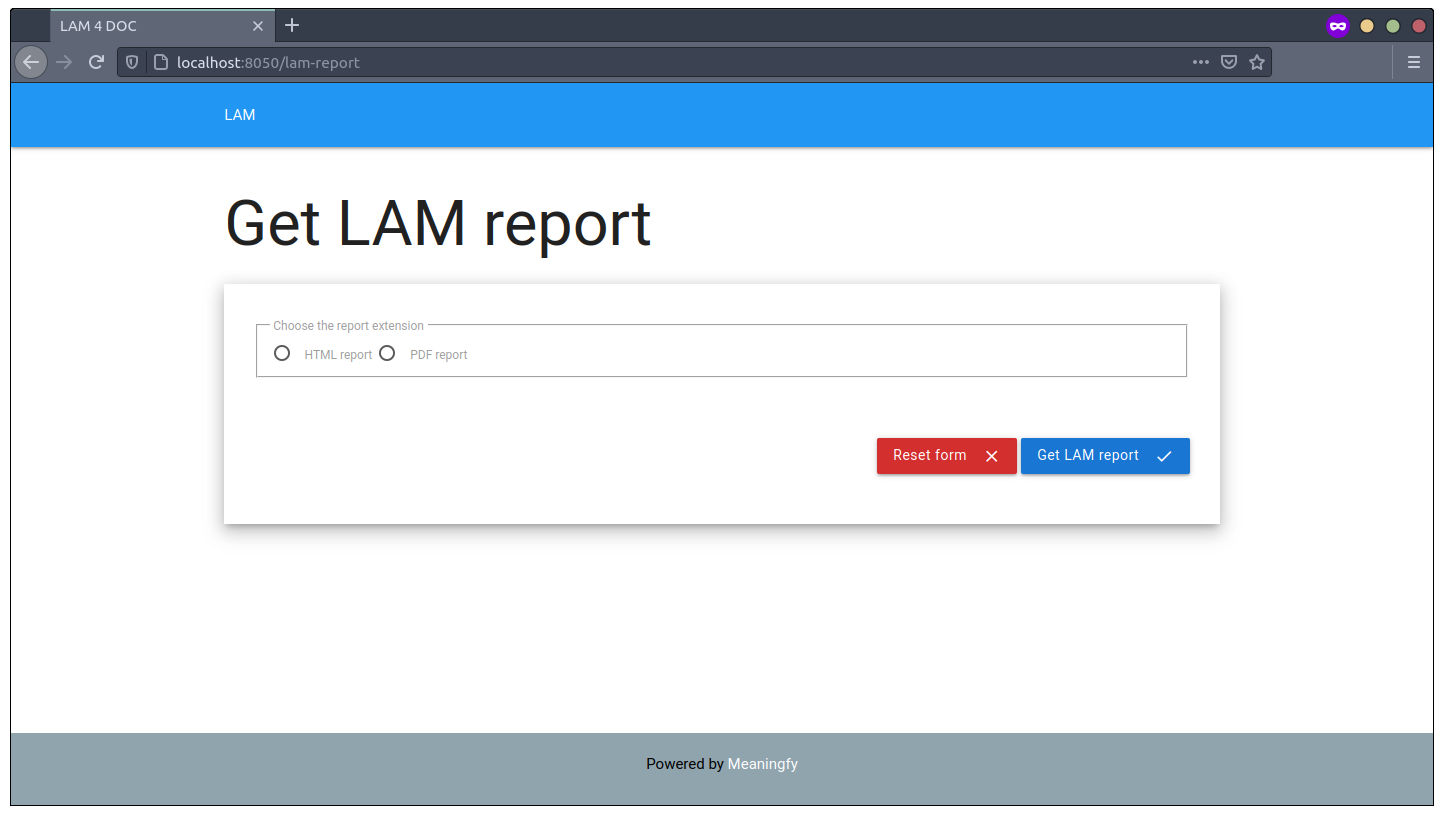
\includegraphics[width=0.9\textwidth]{images/usage/lam-generation-ui-report.png}
  \caption{LAM Generation Services report generation}
  \label{fig:lam-generation-ui-report}
\end{figure} 

To access current tasks and reports, visit the following link\url{http://localhost:8050/tasks}.
Here (Figure \ref{fig:lam-generation-ui-tasks}) you can see a list of tasks and reports that can be downloaded.

\begin{figure}[H]
  \centering
  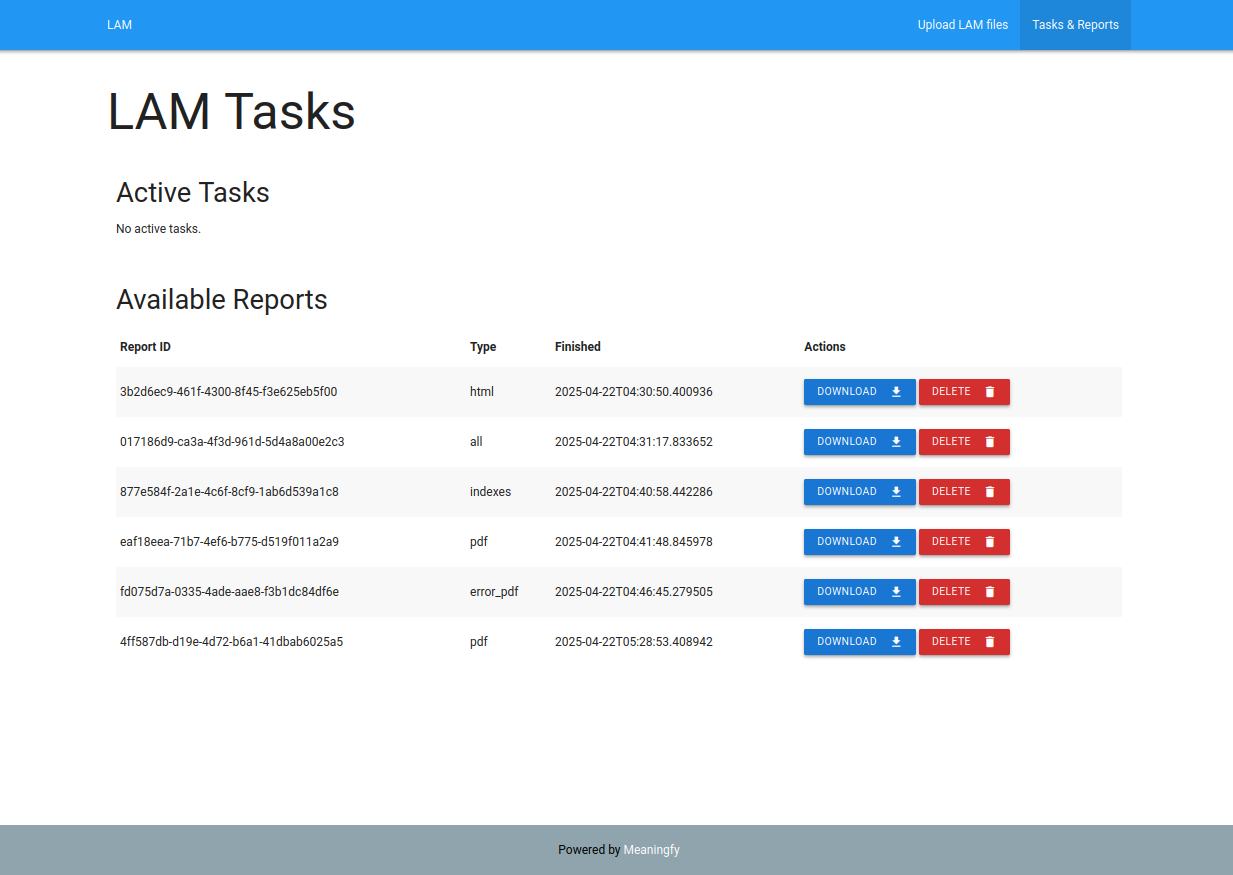
\includegraphics[width=0.9\textwidth]{images/usage/lam-generation-ui-tasks.png}
  \caption{LAM Generation Services tasks page}
  \label{fig:lam-generation-ui-tasks}
\end{figure}

\subsection{LAM Dedicated Triple Store}
To access the LAM Fuseki triple store service visit the following link \url{http://localhost:3010}. You'll be requested the login credentials which can be found in Table \ref{tab:fuseki}. After logging in, you'll be greeted with an interface like in Figure \ref{fig:lam-fuseki-home}.

\begin{figure}[H]
  \centering
  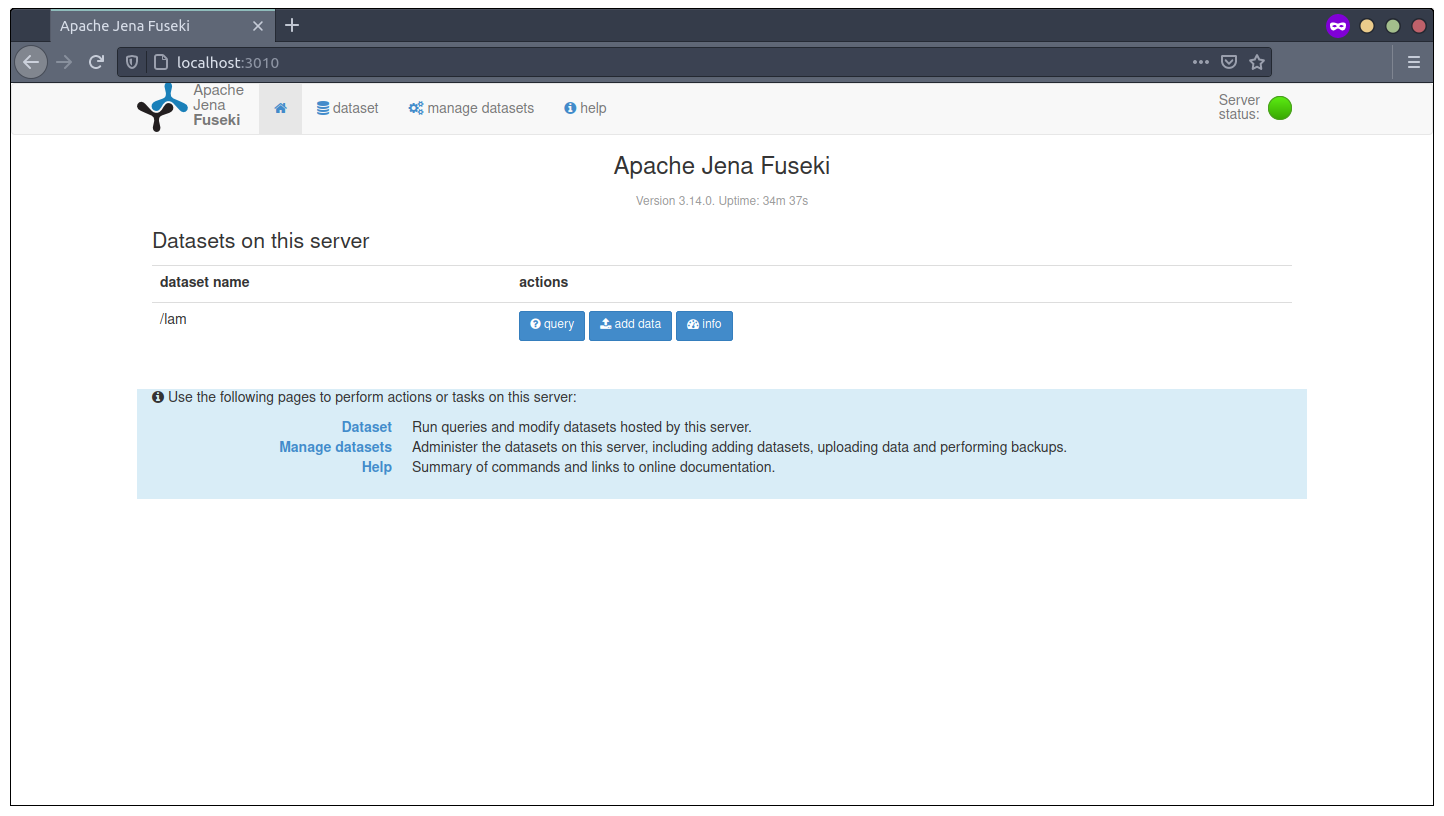
\includegraphics[width=0.9\textwidth]{images/usage/fuseki-home.png}
  \caption{LAM Fuseki home}
  \label{fig:lam-fuseki-home}
\end{figure} 

For more information on how to use Fuseki read the available documentation available at \href{https://jena.apache.org/documentation/fuseki2/}{jena.apache.org}.
\section{Configuration}
\label{sec:configuration}
The deployment suite of micro-services is defined docker-compose.yml file. At deployment and at runtime, the service configurations are provided through OS environment variables available in the \textit{.env} file. The role of the .env file is to enable the system administrators to easily change default configurations as necessary in the context of their environment.

The suite of micro-services is built, started and shut down via docker-compose, a tool designed especially for managing multi-container Docker applications, by describing them in a single file. Then, with a single command, you create and build, start or stop all the services using that configuration file.

In order to avoid hard coding parameters, docker-compose allows you to define them externally. You have the option to define them as operating system level environment variables or provide them in a single file, which is passed as a parameter to the docker-compose tool using the \textit{--env-file} command line argument. Having them in a single file makes much more sense and it is more pragmatic, as you can see and manage all parameters in one place, add the file to the version control system (the contents of the file will evolve and be in sync with the actual code) and have different files for different environments.

The file is usually named \textit{.env} and contains all of the parameters that you want to be able to change and that you need to build and run the defined containers.

Having the parameters in an \textit{.env} file is very useful in a multitude of scenarios, where you would want to have different configurations for different environments where you might want to deploy. As a more specific example, consider a continuous delivery pipeline and the URLs and ports you want your containers to bind (or to connect) to. You thus can easily have two \textit{.env} files, one named \textit{test.env} and one named \textit{acceptance.env}. Each file would have the same declared variables, but with different values for each of the continuous delivery pipeline stage where it’s being deployed. The benefit is that you deploy and test/use the same containers/artifacts and are able to configure them, on the spot, according to the environment that they are integrated with.


Let’s take, for example, the RDF Validator API Docker container, which is defined, in the \texttt{docker-compose.yml} file as it follows:
\begin{lstlisting}[]
lam-validator-api:
	container_name: lam-validator-api
	image: meaningfy/lam-validator-api:latest
	ports:
		- ${RDF_VALIDATOR_API_PORT}:${RDF_VALIDATOR_API_PORT}
	env_file: .env
	restart: always
	networks:
		- mydefault
\end{lstlisting}
The variable used in the definition of this service is just one, \texttt{RDF\_VALIDATOR\_API\_PORT}. And the place where docker-compose will look for that variable is specified in the \texttt{env\_file: .env} line.

Now, if you look in the “.env” file, you will quickly see that the variable is defined as \texttt{RDF\_VALIDATOR\_API\_PORT=10001}. Change the value of the port, rebuild the micro-services and RDF Differ will no longer be listening on \texttt{10001}, but on the new port that you specified.


This section describes the important configurations options available for each of the services.


\subsection{LAM Validator}

LAM validator application exposes an API and an UI and does not depend on any additional services as everything is encapsulated into the Docker image. 

The configuration options are summarised below.

\begin{longtable}[c]{@{}p{4cm}p{5cm}l@{}}
	\toprule
	Description           & Value                   & Associated variable                   \\* \midrule
	\endfirsthead
	%
	\multicolumn{3}{c}%
	{{\bfseries Table \thetable\ continued from previous page}}                             \\
	\endhead
	%
	\bottomrule
	\endfoot
	%
	\endlastfoot
	%
	Validator Service UI port           & 10002                             & \texttt{RDF\_VALIDATOR\_UI\_PORT}      \\
	Validator Service UI location       & http://lam-validator-ui           & \texttt{RDF\_VALIDATOR\_UI\_LOCATION}  \\
	Validator Service API port          & 10001                             & \texttt{RDF\_VALIDATOR\_API\_PORT}     \\
	Validator Service API location      & http://lam-validator-api          & \texttt{RDF\_VALIDATOR\_API\_LOCATION} \\
	\bottomrule
	\caption{LAM Validator configuration}
	\label{tab:validator}                                                                   \\
\end{longtable}

Note, when validating SPARQL endpoints, the fully qualified domain name of the machine must be specified. As a consequence, ``localhost'' domain will not work as expected.

\subsubsection{Configure SHACL Shapes Files}
\label{sec:rdf-validator-ss}
The docker image for the LAM validation API service pulled from \textbf{\href{https://registry.hub.docker.com/r/meaningfy/lam-validator-api}{docker hub}} already contains the required SHACL shape files, as defined in this \textbf{\href{https://github.com/meaningfy-ws/lam-validator/tree/main/resources}{repository}}.

If you want to change the SHACL shapes files, you can use the following customization implemented using \textbf{\href{https://docs.docker.com/storage/volumes/}{docker's volumes}} mechanism. This implementation has been chosen as it requires no in service code modifications from the end-user's side.

An externally defined volume \texttt{rdf-validator-shacl-shapes} which will contain the custom files is coupled with the \texttt{rdf-validator-api} docker container to use when validating. The coupling of the volume to the service container is done with the following statement, which is not included in the default docker compose configuration.

\begin{lstlisting}[]
volumes:
- rdf-validator-shacl-shapes:${RDF_VALIDATOR_SHACL_SHAPES_LOCATION}
\end{lstlisting}

The lines above map the custom shapes that have been copied to the docker volume with the internal location of the container which has been defined in the \texttt{.env} file.

You have to copy these 2 lines in the \texttt{lam-validator-api} container definition in the \texttt{docker-compose.yml} file after the \texttt{image: meaningfy/lam-validator-api:latest} line.

Additionally, the externally defined volume has to be specified in the \texttt{docker-compose.yml} file:
\begin{lstlisting}[]
volumes:
 rdf-validator-shacl-shapes:
  external: true
\end{lstlisting}

To make the custom shapes available to the container create the volume and run the \texttt{make} commands, indicating the location of your shapes through the \texttt{location} variable.
\begin{lstlisting}[language=bash]
make build-volumes
make location=<location to shapes> set-shacl-shapes
\end{lstlisting}

\textbf{NOTE}: Make sure that the location specified ends with a trailing slash \texttt{/}, otherwise the command will not work propery and the templates will not be copied to the docker volume.

Example:
\begin{lstlisting}[language=bash]
make location=/shapes/location/ set-shacl-shapes
\end{lstlisting}

After this, restart the \texttt{lam-validator-api} container for the effects to take place.

\subsection{LAM Generation Service}

LAM Generation Service application exposes an API and an UI for generating the LAM reports (in HTML and PDF formats) and the document index files. It depends on a dedicated triple store which will contain the LAM dataset indicated by the \texttt{LAM\_FUSEKI\_QUERY\_URL} described in table \ref{tab:fuseki} environment variable. 

The configuration options are summarised below.

\begin{longtable}[c]{@{}p{4cm}p{5cm}l@{}}
	\toprule
	Description           & Value                   & Associated variable                   \\* \midrule
	\endfirsthead
	%
	\multicolumn{3}{c}%
	{{\bfseries Table \thetable\ continued from previous page}}                             \\
	\endhead
	%
	\bottomrule
	\endfoot
	%
	\endlastfoot
	%
	LAM Generation Service UI port  & 8050  & \texttt{LAM\_UI\_PORT}             \\	
	LAM Generation Service UI location  & http://lam-generation-service-ui  & \texttt{LAM\_UI\_LOCATION}             \\
	LAM Generation Service API port     & 4050                              & \texttt{LAM\_API\_PORT}                \\
	LAM Generation Service API location & http://lam-generation-service-api & \texttt{LAM\_API\_LOCATION}            \\
	\bottomrule
	\caption{LAM Generation Service configuration}
	\label{tab:lam-generation}                                                                   \\
\end{longtable}

\subsection{LAM dedicated triple store}
	
LAM Generation Services depends on a Fuseki triple store and query the data required for the LAM reports and index files.

The available configurations are described below. 

\begin{longtable}[c]{@{}p{4cm}p{5cm}l@{}}
	\toprule
	Description & Value & Associated variable \\* \midrule
	\endfirsthead
	%
	\multicolumn{3}{c}%
	{{\bfseries Table \thetable\ continued from previous page}} \\
	\endhead
	%
	\bottomrule
	\endfoot
	%
	\endlastfoot
	%
	Admin account password & admin & \texttt{LAM\_FUSEKI\_ADMIN\_PASSWORD} \\
	User name & admin & \texttt{LAM\_FUSEKI\_USERNAME} \\
	Password & admin & \texttt{LAM\_FUSEKI\_PASSWORD} \\
	Folder where Fuseki stores data & ./data/diff & \texttt{LAM\_FUSEKI\_DATA\_FOLDER} \\
	Additional arguments passed to JVM & -Xmx2g & \texttt{LAM\_FUSEKI\_JVM\_ARGS} \\
	URL & http://rdf-differ-fuseki & \texttt{LAM\_FUSEKI\_LOCATION} \\
	LAM Fuseki port                     & 3030                              & \texttt{LAM\_FUSEKI\_PORT}             \\
	LAM Fuseki External port            & 3010                              & \texttt{LAM\_FUSEKI\_EXTERNAL\_PORT}   \\
	LAM Fuseki location                 & http://lam-fuseki                 & \texttt{LAM\_FUSEKI\_LOCATION}     \\
	Fuseki LAM dataset location                  & \texttt{/lam/query}
	& \texttt{LAM\_FUSEKI\_QUERY\_URL}     \\* \bottomrule
	\caption{LAM Generation Services dedicated triple store configuration}
	\label{tab:fuseki}\\
\end{longtable}
\section{Makefile targets}
\label{sec:makefile_targets}
	Makefile targets provide a convenient and easy way of running different tools that the software packages provide. The usage is \textbf{make \textit{target}}.
	
	Following is a list of available targets along with the description.

\begin{itemize}
	\item \textbf{install}
	- Upgrades PIP to the latest version and installs the local requirements
	
	\item \textbf{test}
	- Runs pytest which in turns executes the unit and BDD tests which are ran using headless Chrome. You need to successfully run the \textbf{install} target beforehand, as it installs the necessary prerequisites (the chrome browser and the driver which corresponds to that specific chrome browser version)
	
	\item \textbf{test-with-ui}
	- Runs pytest which in turns executes the unit and BDD tests which are ran using the fully UI enabled Chrome. You need to successfully run the \textbf{install} target beforehand, as it installs the necessary prerequisites (the chrome browser and the driver which corresponds to that specific chrome browser version). A "Chrome is being controlled by automated test software" message will be displayed on the top. Please wait for the tests to finish and do not interact with the browser window(s) driven by the BDD tests. 
	
	\item \textbf{build-services}
	- Uses docker-compose to build all the services defined in the docker/docker-compose.yml file.
	
	\item \textbf{start-services}
	- Uses docker-compose to start the services defined in the docker/docker-compose.yml file.
	
	\item \textbf{stop-services}
	- Uses docker-compose to stop the services defined in the docker/docker-compose.yml file.
	
	\item \textbf{generate-indexes}
	- Uses \href{https://pypi.org/project/eds4jinja2/}{eds4jinja2} to generate the indexes that will later be sent to ElasticSearch for indexing.
	
	\item \textbf{generate-content}
	- Uses \href{https://pypi.org/project/eds4jinja2/}{eds4jinja2} to generate the content that will be integrated in the portal.
	
	\item \textbf{generate-tests-from-features}
	- Based on the feature files, this target generates the missing Python test code.
\end{itemize}
\section{Indexes fields}
\label{sec:indexes_fields}
\begin{enumerate}
	\item CELEX
	\begin{itemize}
		\item \textbf{classURI}: The URI of the class (for example \lstinline!http://publications.europa.eu/resources/authority/lam/c_108!)
		\item \textbf{types}: The RDF type(s) ( for example \lstinline!http://www.w3.org/2004/02/skos/core#Concept! )
		\item \textbf{authors}: The author(s) of the current class (for example \lstinline!http://publications.europa.eu/resource/authority/corporate-body/CONSIL!)
		\item \textbf{resourceTypes}: The resource type (for example \lstinline!http://publications.europa.eu/resource/authority/resource-type/STRATEGY_COMMON!). This is also known as the type of act (\lstinline!lamd:md_fm\endverbatim!).
		\item \textbf{collections}: The collection that the current class is part of (for example \lstinline!http://publications.europa.eu/resources/authority/lam/class_3OTHER!)
		\item \textbf{dnClassValues}: Class or subclass according to CDM.
		\item \textbf{dc}: The Eurovoc concept for this specific class.
		\item \textbf{ct}: The subject matter concept for this specific class.
		\item \textbf{cc}: The directory code for this specific class.
		\item \textbf{labels}: The label(s) of the current class (for example "Common strategy , Common strategy , Common strategy , Common strategy (CFSP number), Common strategy (CFSP number), Common strategy (CFSP number)")
		\item \textbf{notes}: The notes of the current class (for example \lstinline!"Proposal: strategy_council."!)
		\item \textbf{examples}: The examples for the current class (for example "32003E0897, Common Strategy 2003/897/CFSP of the European Council of 12 December 2003 amending Common Strategy 1999/877/CFSP on Ukraine in order to extend the period of its application , Stratégie commune 2003/897/PESC du Conseil européen du 12 décembre 2003 modifiant la stratégie commune 1999/877/PESC à l'égard de l'Ukraine afin de proroger sa période d'application, 32003E0897, Common Strategy 2003/897/CFSP of the European Council of 12 December 2003 amending Common Strategy 1999/877/CFSP on Ukraine in order to extend the period of its application , Stratégie commune 2003/897/PESC du Conseil européen du 12 décembre 2003 modifiant la stratégie commune 1999/877/PESC à l'égard de l'Ukraine afin de proroger sa période d'application")
	\end{itemize}
	\item Classes
	\begin{itemize}
	\item \textbf{classURI}: The URI of the class (for example \lstinline!http://publications.europa.eu/resources/authority/lam/c_108!)
	\item \textbf{types}: The RDF type(s) ( for example \lstinline!http://www.w3.org/2004/02/skos/core#Concept! )
	\item \textbf{AU}: The author(s) of the current class (for example \lstinline!http://publications.europa.eu/resource/authority/corporate-body/CONSIL!)
	\item \textbf{FM}: The resource type (for example \lstinline!http://publications.europa.eu/resource/authority/resource-type/STRATEGY_COMMON!). This is also known as the type of act (\lstinline!lamd:md_fm!).
	\item \textbf{collections}: The collection that the current class is part of (for example \lstinline!http://publications.europa.eu/resources/authority/lam/class_3OTHER!)
	\item \textbf{\lstinline!CDM_CLASS!}: Class or subclass according to CDM.
	\item \textbf{DC}: The Eurovoc concept for this specific class.
	\item \textbf{CT}: The subject matter concept for this specific class.
	\item \textbf{CC}: The directory code for this specific class.
	\item \textbf{\lstinline!DN_CLASS!}: The CELEX class.
	\item \textbf{labels}: The label(s) of the current class (for example "Common strategy , Common strategy , Common strategy , Common strategy (CFSP number), Common strategy (CFSP number), Common strategy (CFSP number)")
	\item \textbf{notes}: The notes of the current class (for example \lstinline!"Proposal: strategy_council."!)
	\item \textbf{examples}: The examples for the current class (for example "32003E0897, Common Strategy 2003/897/CFSP of the European Council of 12 December 2003 amending Common Strategy 1999/877/CFSP on Ukraine in order to extend the period of its application , Stratégie commune 2003/897/PESC du Conseil européen du 12 décembre 2003 modifiant la stratégie commune 1999/877/PESC à l'égard de l'Ukraine afin de proroger sa période d'application, 32003E0897, Common Strategy 2003/897/CFSP of the European Council of 12 December 2003 amending Common Strategy 1999/877/CFSP on Ukraine in order to extend the period of its application , Stratégie commune 2003/897/PESC du Conseil européen du 12 décembre 2003 modifiant la stratégie commune 1999/877/PESC à l'égard de l'Ukraine afin de proroger sa période d'application")
	\end{itemize}
	\item Properties
	\begin{itemize}
		\item \textbf{propertyURI}: The URI of the property (for example \lstinline!http://publications.europa.eu/resources/authority/lam/md_SUSPEND_PAR!)
		\item \textbf{types}: The URI of the type of the property (for example \lstinline!http://www.w3.org/2004/02/skos/core#Concept!) 
		\item \textbf{propertyCollections}: The URI(s) of the collection(s) that the property is part of (for example \lstinline!http://publications.europa.eu/resources/authority/lam/class_MSEA!)
		\item \textbf{propertyCollectionLabels}: The label(s) of the collections that the property is part of (for example "Amendment to/Earlier related instruments")
		\item \textbf{propertyTypes}: The type(s) of the property (for example "object property")
		\item \textbf{skosDefinitions}: The SKOS definition(s) of the property (for example "Partial suspension (SP) - similar as Suspension")
		\item \textbf{editorialNotes}: The editorial notes for the property (for example "08/11/2019: Diferences between suspension and partial suspension? Is this really needed?")
		\item \textbf{examples}: The examples for the property (for example \lstinline!"<j.0:resource_legal_term-of-office rdf:datatype=\"http://www.w3.org/2001/XMLSchema#string\">VII (2020-2025)</j.0:resource_legal_term-of-office>"!)
		\item \textbf{historyNotes}: The history notes for the property (for example "Used by EUR-Lex quick search. Relevant for search in internal numbers for ECB, therefore this property is created in some ECB documents on purpose.")
		\item \textbf{scopeNotes}: The scope notes for the property (for example "32013R0298 → 32004R0314")
		\item \textbf{notations}: The notations for the property (for example \lstinline!"SUSPEND_PAR"!) 
		\item \textbf{labels}: The labels for the property (for example "Link: Partially suspends document")
	\end{itemize}
\end{enumerate}

\newpage
\section*{Appendices}
\addcontentsline{toc}{section}{\bfseries Appendices}
\renewcommand{\thesubsection}{\arabic{subsection}}
\setcounter{subsection}{0}% Restart subsection numbering

\input{content/appendinx.tex}

\bibliography{../references/references.bib}

\end{document}

%This template was created by Roza Aceska.
